\section{Introduction}
\label{sec:intro}
\acp{ICD} are life-saving medical devices.
An \ac{ICD} is implanted under the shoulder, and connects directly to the heart muscle though two electrodes and continuously measures the heart's rhythm (Fig. \ref{fig:icd}).
If it detects a potentially fatal accelerated rhythm known as Ventricular Tachycardia (VT), the \ac{ICD} delivers a high-energy electric shock or sequence of pulses through the electrodes to reset the heart's electrical activity.
Without this therapy, the VT can be fatal within seconds of onset.
In the US alone, 10,000 people receive an \ac{ICD} every month.
Studies have presented evidence that patients implanted with \acp{ICD} have a mortality rate reduced by up to 31\%.

Unfortunately, \acp{ICD} suffer from a high rate of \emph{inappropriate therapy} due to poor detection of the current rhythm on the part of the \ac{ICD}.
In particular, a class of rhythms known as SupraVentricular Tachycardias (SVTs) can fool the detection algorithms.
Inappropriate shocks increase patient stress, reduce their quality of life, and are linked to increased morbidity.
Depending on the particular ICD and its settings, the rates of inappropriate therapy can range from 46\% to 62\% of all delivered therapy episodes.
Current practice for \ac{ICD} verification relies heavily on testing and software cycle reviews.
With the advent of computer models of the human heart, \emph{Model-Based Design} (MBD) can supply rigorous evidence of safety and efficacy. 
This paper presents hybrid system models of the human heart and of the common modules of \acp{ICD} currently on the market, and shows that the closed loop formed by these models admits a finite bisimulation.
The objective is to develop model checkers for \acp{ICD} to further their MBD process.
\begin{figure}[t]
	\centering
	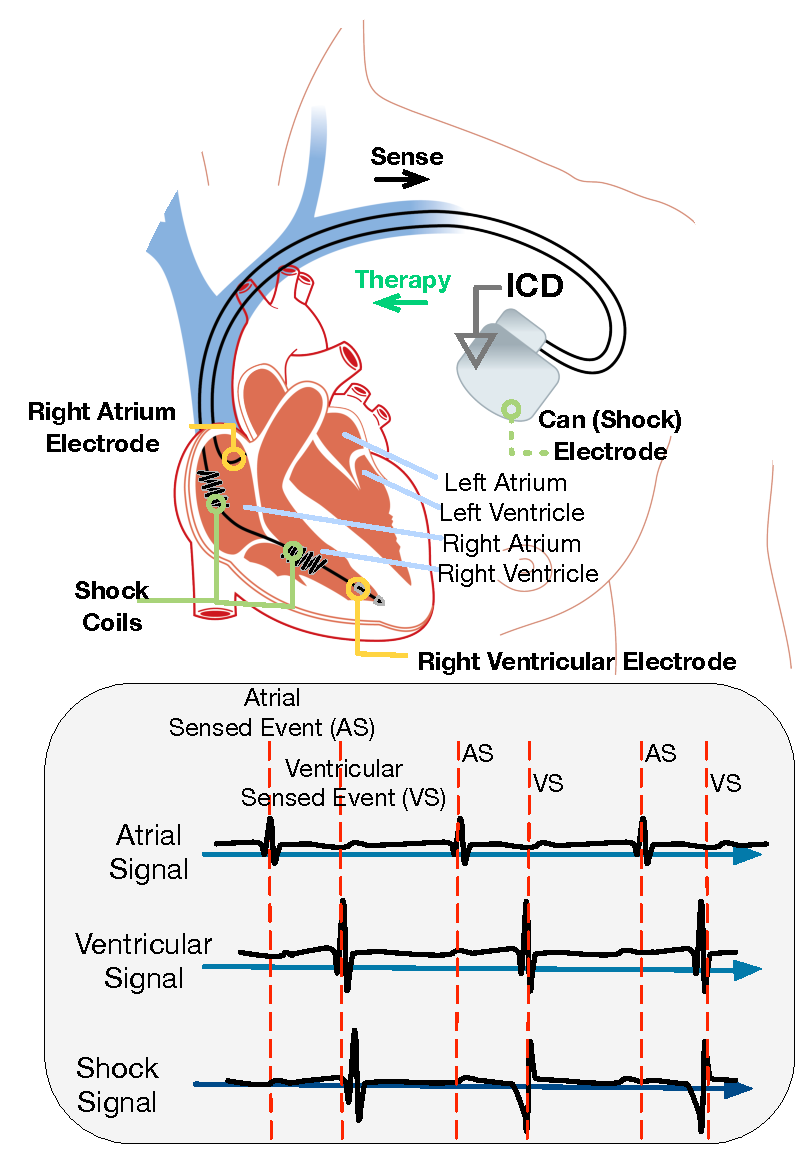
\includegraphics[scale=0.3]{figures/figICD}
	\vspace{-10pt}
	\caption{\small ICD connected to a human heart via two electrodes. The ICD monitors three electrical signals (known as electrograms) traversing the heart muscle.}
	\label{fig:icd}
	\vspace{-10pt}
\end{figure}

\begin{figure*}[t]
	\centering
	\vspace{-10pt}
	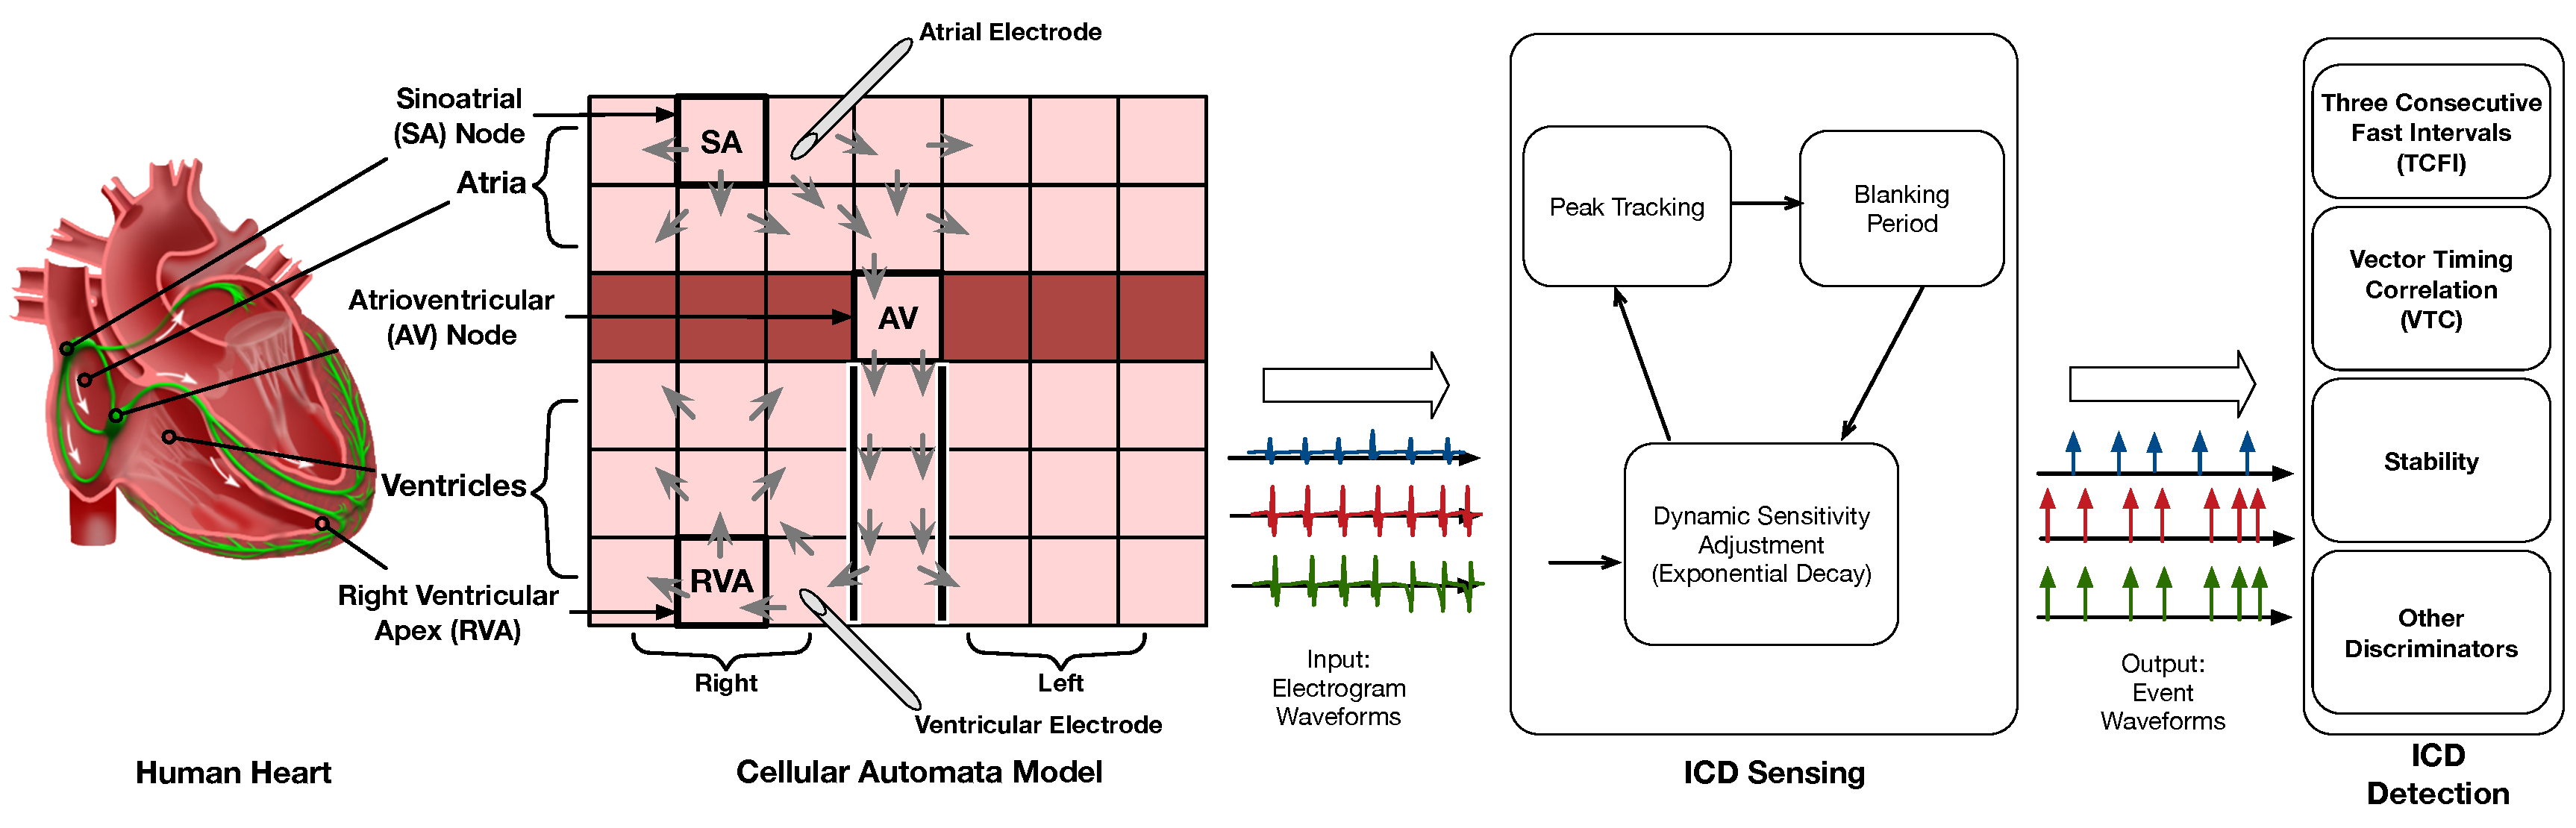
\includegraphics[scale=0.28]{figures/overviewFigure}
	\vspace{-10pt}
	\caption{\small The whole heart is modeled as a 2D mesh of cells (Section \ref{sec:heartcellularautomata}). The \ac{ICD} electrodes are shown in the right atrium and ventricle. The electrogram signals measured through the electrodes are processed by the sensing module (see Section \ref{sec:sensing}). The detection algorithm determines the current rhythm using the processed signal (Section \ref{sec:discriminators}).}
	\label{fig:overview}
	\vspace{-10pt}
\end{figure*}
No work exists on \ac{ICD} verification. 
Earlier work on verification of medical devices (formal or otherwise) focuses on pacemakers.
\ac{ICD} algorithms are more complex than a pacemaker's: an \ac{ICD} measures the timing of events, but also measures and processes the \emph{morphology} of the electrical signal in the heart to distinguish many types of arrhythmias.
This takes the model out of the realm of timed automata and into hybrid automata proper.

The first contribution of this paper is to develop a hybrid system model of the heart and \ac{ICD} measurement process (Section \ref{sec:heartcellularautomata}), 
of the sensing process (Section \ref{sec:sensing}),
and of the algorithmic components of \acp{ICD} from most major manufacturers on the market (Section \ref{sec:discriminators}, \yhl{see Fig.~\ref{fig:overview}}).
We show that the composition of these three models admits a finite bisimulation.
The \ac{ICD} models presented here are the first formalization of \ac{ICD} operation to the best of our knowledge.
To establish this result we use the theory of STORMED hybrid systems \cite{VladimerouPVD08_STORMED}, a class of hybrid systems that have finite bisimulations.
Our second contribution is two general results for STORMED systems.
First we prove that parallel compositions of STORMED systems yield STORMED systems (Section \ref{sec:compositionality}).
Secondly, we show that any definable over-approximate reach tubes can replace the exact trajectories of a STORMED system, yielding a system that still admits a finite \emph{simulation} (Section \ref{sec:simulationAprox}). 
